\documentclass[a4paper,11pt]{article}

\usepackage[T1]{fontenc}
\usepackage[swedish]{babel} 
\usepackage[utf8]{inputenc}
\usepackage{graphicx}
\usepackage{placeins}

\usepackage{fancyhdr}
\pagestyle{fancy}

\fancyhead{}
\fancyfoot{}

\fancyhead[L]{Grafer och planäritet}
\fancyhead[R]{Peter Boström -- \emph{pbos@kth.se}}
\fancyfoot[C]{Diskret matematik, SF1631}
\fancyfoot[R] {\thepage}

\title{Grafer och planäritet\\\vspace{4pt}\normalsize Derp derp undertitel hej.}
\author{Peter Boström -- \emph{pbos@kth.se}}

\begin{document}
\maketitle
\pagestyle{fancyplain}

\section*{Grafer, kompletta grafer och andra begrepp}

En \textbf{graf} är en samling, eller \emph{mängd}, av så kallade \emph{noder} och \emph{kanter} mellan dem. En nod är en punkt och en kant är ett sträck draget mellan två noder. En kant är en anslutning mellan två noder.

\begin{figure}[!ht]
	\begin{center}
		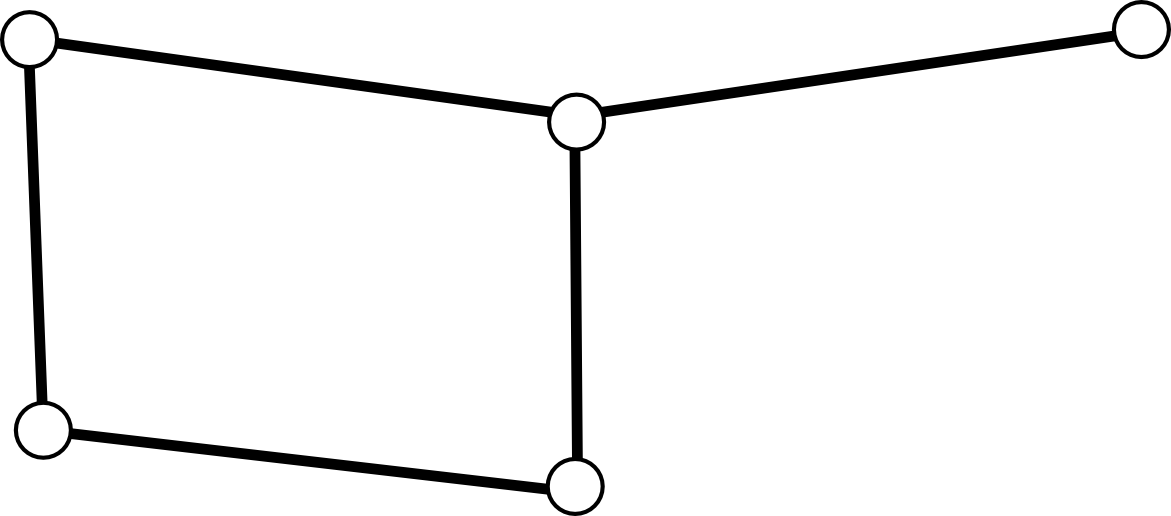
\includegraphics{fig1}
		\caption{En graf med 5 noder och 5 kanter.}
		\label{fig1}
	\end{center}
\end{figure}
\FloatBarrier

En \textbf{bipartit graf} är en graf där grafen kan delas upp i två grupper av noder som inte har några kanter internt mellan sig, men tillåts ha anslutningar mellan noder som inte tillhör samma grupp.

\begin{figure}[!ht]
	\begin{center}
		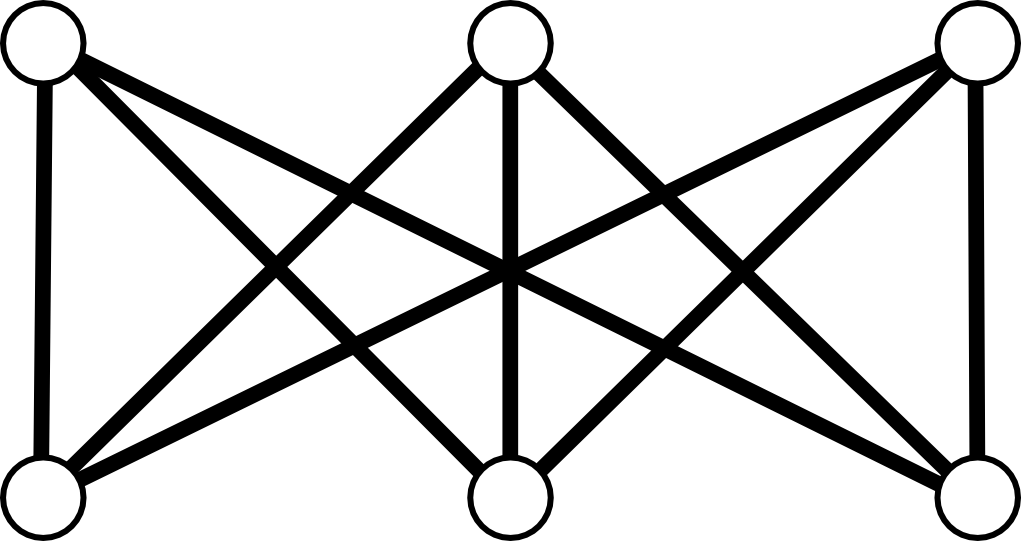
\includegraphics{fig2}
		\caption{Bipartit graf med två grupper om 3 noder vardera.}
		\label{fig2}
	\end{center}
\end{figure}
\FloatBarrier

En \textbf{komplett graf} är en graf där varje par av noder har en kant mellan sig. Kompletta grafer tecknas $K_n$ där $n$ är antalet noder.

\begin{figure}[!ht]
	\begin{center}
		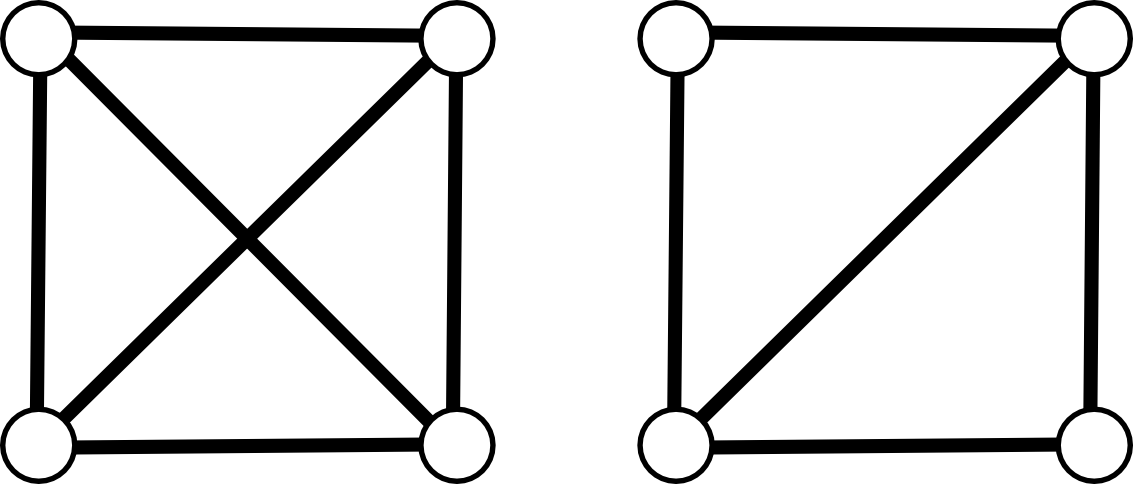
\includegraphics{fig3}
		\caption{Blah stuff figure shit.}
		\label{fig3}
	\end{center}
\end{figure}
\FloatBarrier

$$bild\ k_4,\ bild\ k_4-\{e\}$$

Bildförklaring sista bilden. Den högra är inte komplett då det saknas en kant mellan nod $blah_1$ och $blah_2$.

\textbf{Kompletta bipartita grafer} tecknas $K_{n,m}$ och har två grupper av noder med $n$ respektive $m$ stycken noder där varje nod ansluter till varje enskild nod i den andra gruppen. Figur \cite{fig2} är ett exempel på en komplett bipartit graf, $K_{3,3}$.

\section*{Grafers planäritet}

En graf är \textbf{plan} om blah blah ritad på ett visst sätt.

\begin{figure}[!ht]
	\begin{center}
		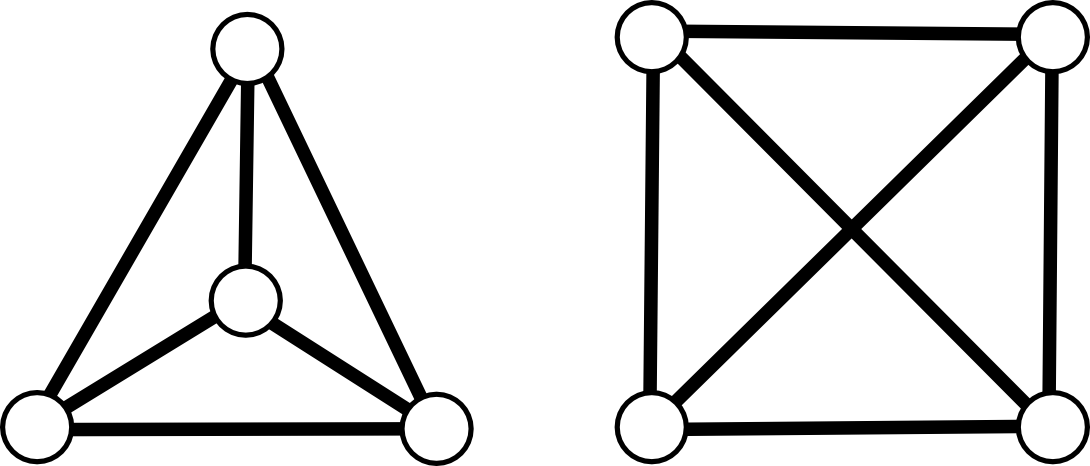
\includegraphics{fig4}
		\caption{Blah stuff figure shit.}
		\label{fig4}
	\end{center}
\end{figure}
\FloatBarrier

$$bild\ k_4\ plan,\ bild\ k_4$$

Båda grafer bildar den kompletta grafen $K_4$. Den vänstra grafen är plant ritad medan den högra inte är det då (minst) två kanter korsar varandra.
Bildförklaring, vänsterbilden plan medan högerbilden inte är det då (minst) två kanter korsar varandra.

En \textbf{planär graf} är en graf som \emph{kan} ritas så, men behöver nödvändigtvis inte vara ritad så. I exemplet ovan, figur \cite{somefig}, är endast den vänstra grafen plan medan båda grafer är planära.

Grafers planäritet har viktiga verkliga användningsområden. Ett vanligt exempel är vid konstruktion av kretskort BLAH MROE STUFF HERE.
Varför viktigt? Blah blah kretskort jag har ingen kreativitet mer än så. En plan graf är även ofta mer lättläst än andra som blir mer sammannystade då kanter korsar varandra.

\section*{Ickeplanära grafer}

Grafer som inte går att rita plant kallas för \textbf{ickeplanära grafer}. Ett exempel på en ickeplanär graf är kompletta grafen med 5 noder, $K_5$.

\begin{figure}[!ht]
	\begin{center}
		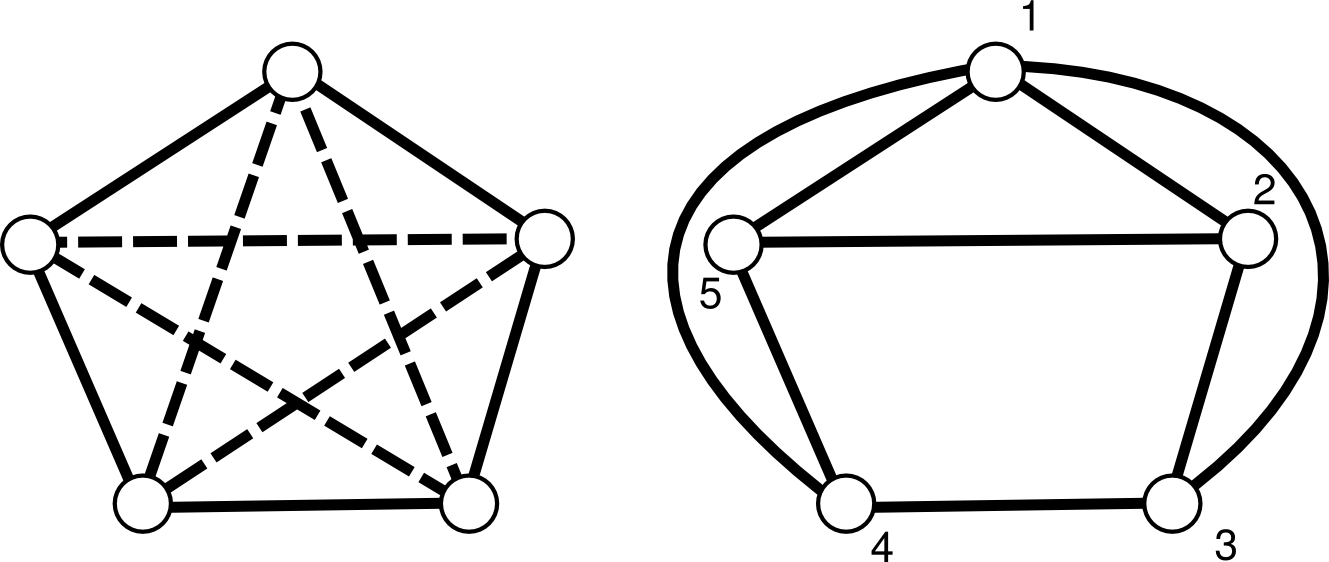
\includegraphics{fig5}
		\caption{Blah stuff figure shit.}
		\label{fig5}
	\end{center}
\end{figure}
\FloatBarrier

$$Bilden,\ studiematerialet, K_5$$

*Intuitiv förklaring till bilden, att linjer måste ritas inuti eller utanför pentagonen helt för att inte korsa andra linjer.*

Då $K_4$ som tidigare nämnts är planär är $K_5$ den minsta kompletta grafen som samtidigt inte är planär.

En annan graf som inte går att rita plant är $K_{3,3}$.

\begin{figure}[!ht]
	\begin{center}
		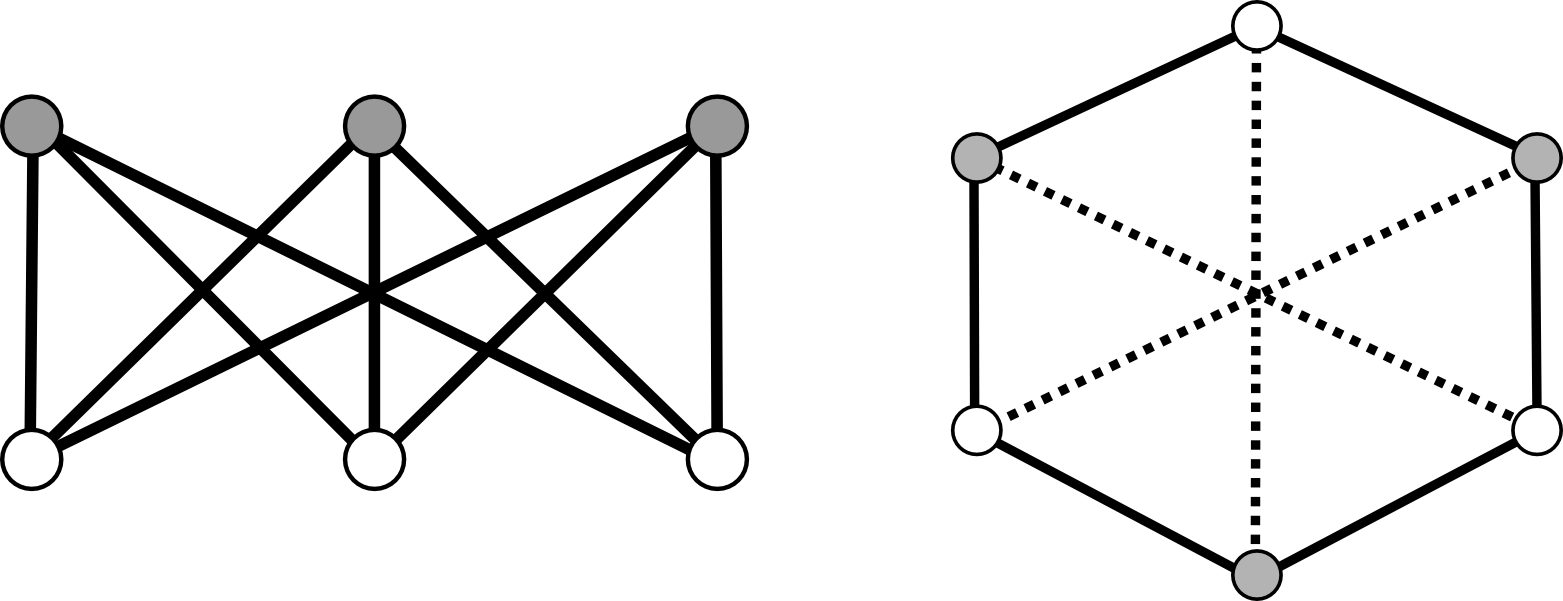
\includegraphics{fig6}
		\caption{Blah stuff figure shit.}
		\label{fig6}
	\end{center}
\end{figure}
\FloatBarrier

$$bild\ K_{3,3},\ bild\ K_{3,3}\ som\ hexagon$$

Förklaring till varför $K_{3,3}$ inte är planär. Blah blah ritas utanför /eller/ inuti.

$K_{2,3}$ däremot är planär och $K_{3,3}$ är på liknande sätt den minsta kompletta bipartita grafen. 

\begin{figure}[!ht]
	\begin{center}
		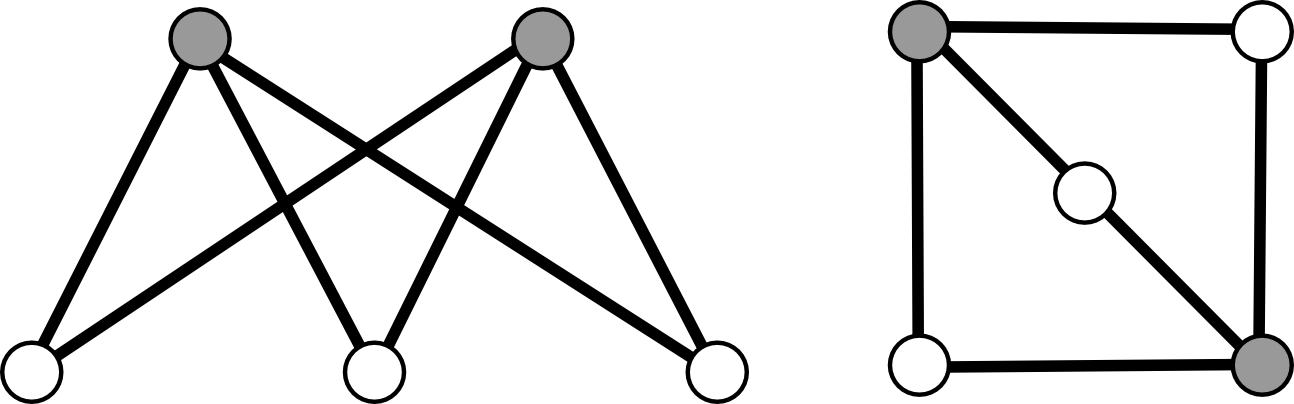
\includegraphics{fig7}
		\caption{Blah stuff figure shit.}
		\label{fig7}
	\end{center}
\end{figure}
\FloatBarrier

$$bild\ K_{2,3},\ bild\ K_{2,3}\ plan$$

\section*{Homomorfa grafer och större ickeplanära grafer}

Vad är en homomorf graf? Förklara iaf. hur det är relevant för vårat fall.

\begin{figure}[!ht]
	\begin{center}
		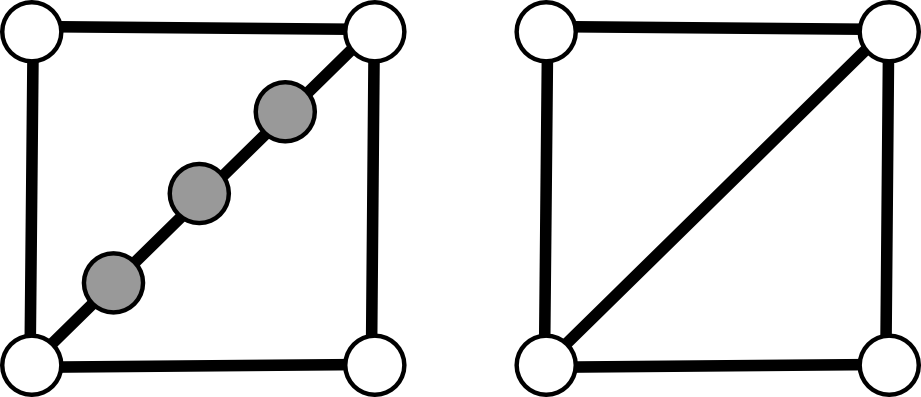
\includegraphics{fig8}
		\caption{Blah stuff figure shit.}
		\label{fig8}
	\end{center}
\end{figure}
\FloatBarrier

$$bilden\ från\ 12.5\ studiematerialet$$

Förklara varför det inte påverkar planäriteten av grafen och att de därför är identiska så vitt vi bryr oss. Varje graf är även homomorf med sig själv.

Det har visat sig att ingen planär graf har en delgraf (kan vara hela grafen) som är homomorf med $K_{5}$ eller $K_{3,3}$. Detta påstående kallas för Kuratowskis teorem. Bevis för detta teorem finns men är komplicerat och lämnas åt den intresserade läsaren att finna.

Varje graf är planär enbart om det inte finns en delgraf som går att sammandra till $K_5$ eller $K_{3,3}$. Förklara sammandragningar ish. "Som kan representeras, utan att fuska\texttrademark, med ett hörn".

\begin{figure}[!ht]
	\begin{center}
		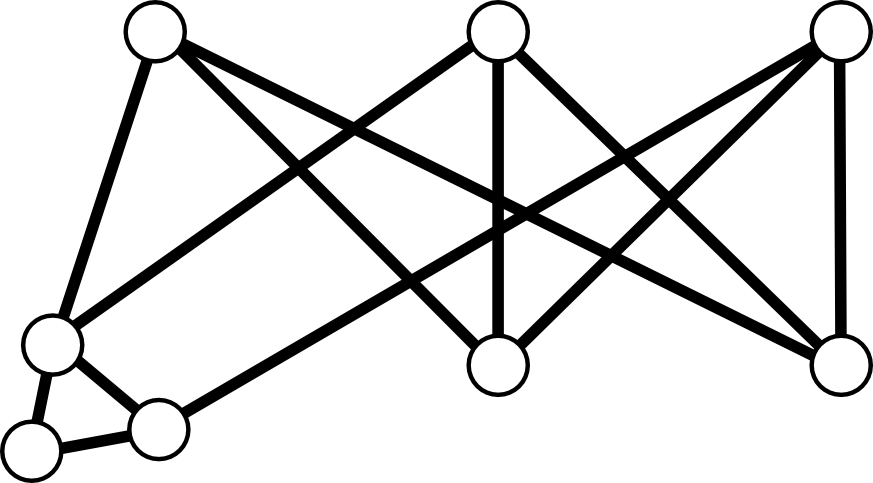
\includegraphics{fig9}
		\caption{Blah stuff figure shit.}
		\label{fig9}
	\end{center}
\end{figure}
\FloatBarrier

$$bild\ 12.6\ looks\ nice.$$

Förklara bilden och att det är en sammandragning av en planär delgraf som inte skapar konflikter inuti noden.

Exempel på en ickeplanär graf som inte direkt är $K_{3,3}$ men går att dra samman till den.

\end{document}

